\section{Exceptions}
Exceptions sind Ausnahmefälle welche durch den \textit{try-catch}-Block abgefangen werden können. Es gibt in Java zwei unterschiedliche Arten von Exceptions: 
\begin{itemize}[nosep]
	\item Error
	\item Exception
\end{itemize}

\noindent Dabei sind \textbf{Error} schwerwiegende Fehler die \underline{nicht behandlet} werden sollen zB OutOfMemoryError, StackOverflowError etc. Hingegen sind \textbf{Exception} Laufzeitfehler die \underline{behandelbar} sind zB IOException.


\subsection{Unchecked vs Checked}
In Java müssen alle Exceptions welche eine checked Objekt werfen, diese in der Deklaration beinhalten bzw werden vom Kompiler geprüft. Unchecked Exceptions sind RuntimeExceptions sowie Error und deren Unterklassen welche nicht vom Kompiler geprüft werden. 
\begin{lstlisting}
static String readFile(String path) throws IOException {
	if (path == null) throw new NullPointerException("No Path");
	
	throw new IOException("Not implemented yet");
}

void testMethod() {
	try {
		readString("test.txt");
	} catch (IOException | NullPointerException e) {
		e.printStackTrace();
	} finally {
		System.out.println("Finished");
	}
}
\end{lstlisting}
\begin{center}
	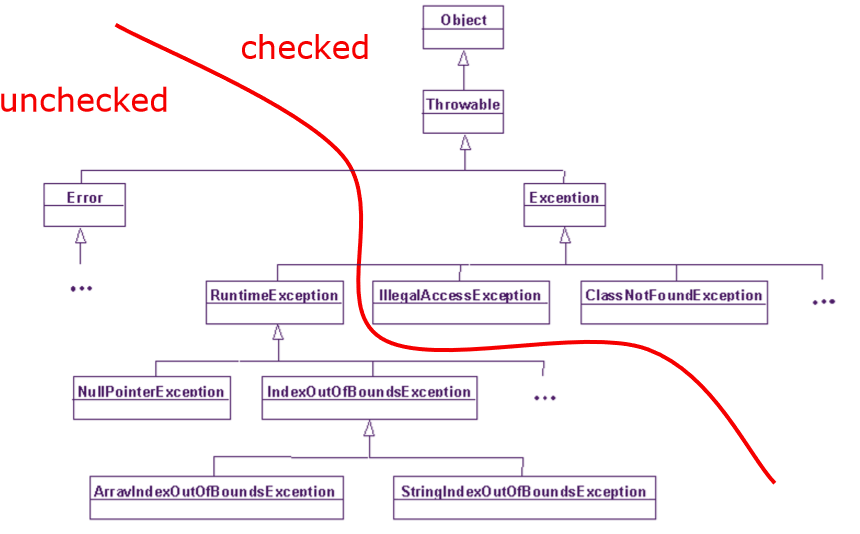
\includegraphics[width= 0.8\columnwidth]{Images/exception_uc}
\end{center}

\subsection{Resources}
Wenn eine Klasse \textit{AutoClosable} implementiert, kann sie automatisch geschlossen werden mit einem Try-With-Resources block
\begin{lstlisting}
try (Scanner s = new Scanner(System.in)) {
	// work with s
}
\end{lstlisting}